\chapter{Задание}

Построить схему выполнения системного вызова open в зависимости от значения основных флагов определяющих открытие файла на чтение, на запись, на выполнение и на создание нового файла. В схеме должны быть названия функций и кратко указаны выполняемые ими действия. По ГОСТу это делается с помощью выносных линий в фигурных скобках.

В схему нужно обязательно включить следующие действия, выполняемые соответствующими функциями ядра:

\begin{enumerate}[label=\arabic*)]
    \item копирование названия файла из пространства пользователя в пространство ядра;
\item блокировка/разблокировка (spinlock) структуры files\_struct и других действий в разных функциях;
    \item алгоритм поиска свободного дескриптора открытого файла;
    \item работу со структурой nameidata – инициализация ее полей;
    \item алгоритм разбора пути (кратко);
    \item инициализацию полей struct file;
    \item «открытие» файла для чтения, записи или выполнения;
    \item создание inode в случае отсутствия открываемого файла.
Отчет должен включать: титульный лист и схему алгоритма работы
системного вызова open.
\end{enumerate}

\chapter{Схема}

\begin{figure}[H]
    \centering
    \caption{}
    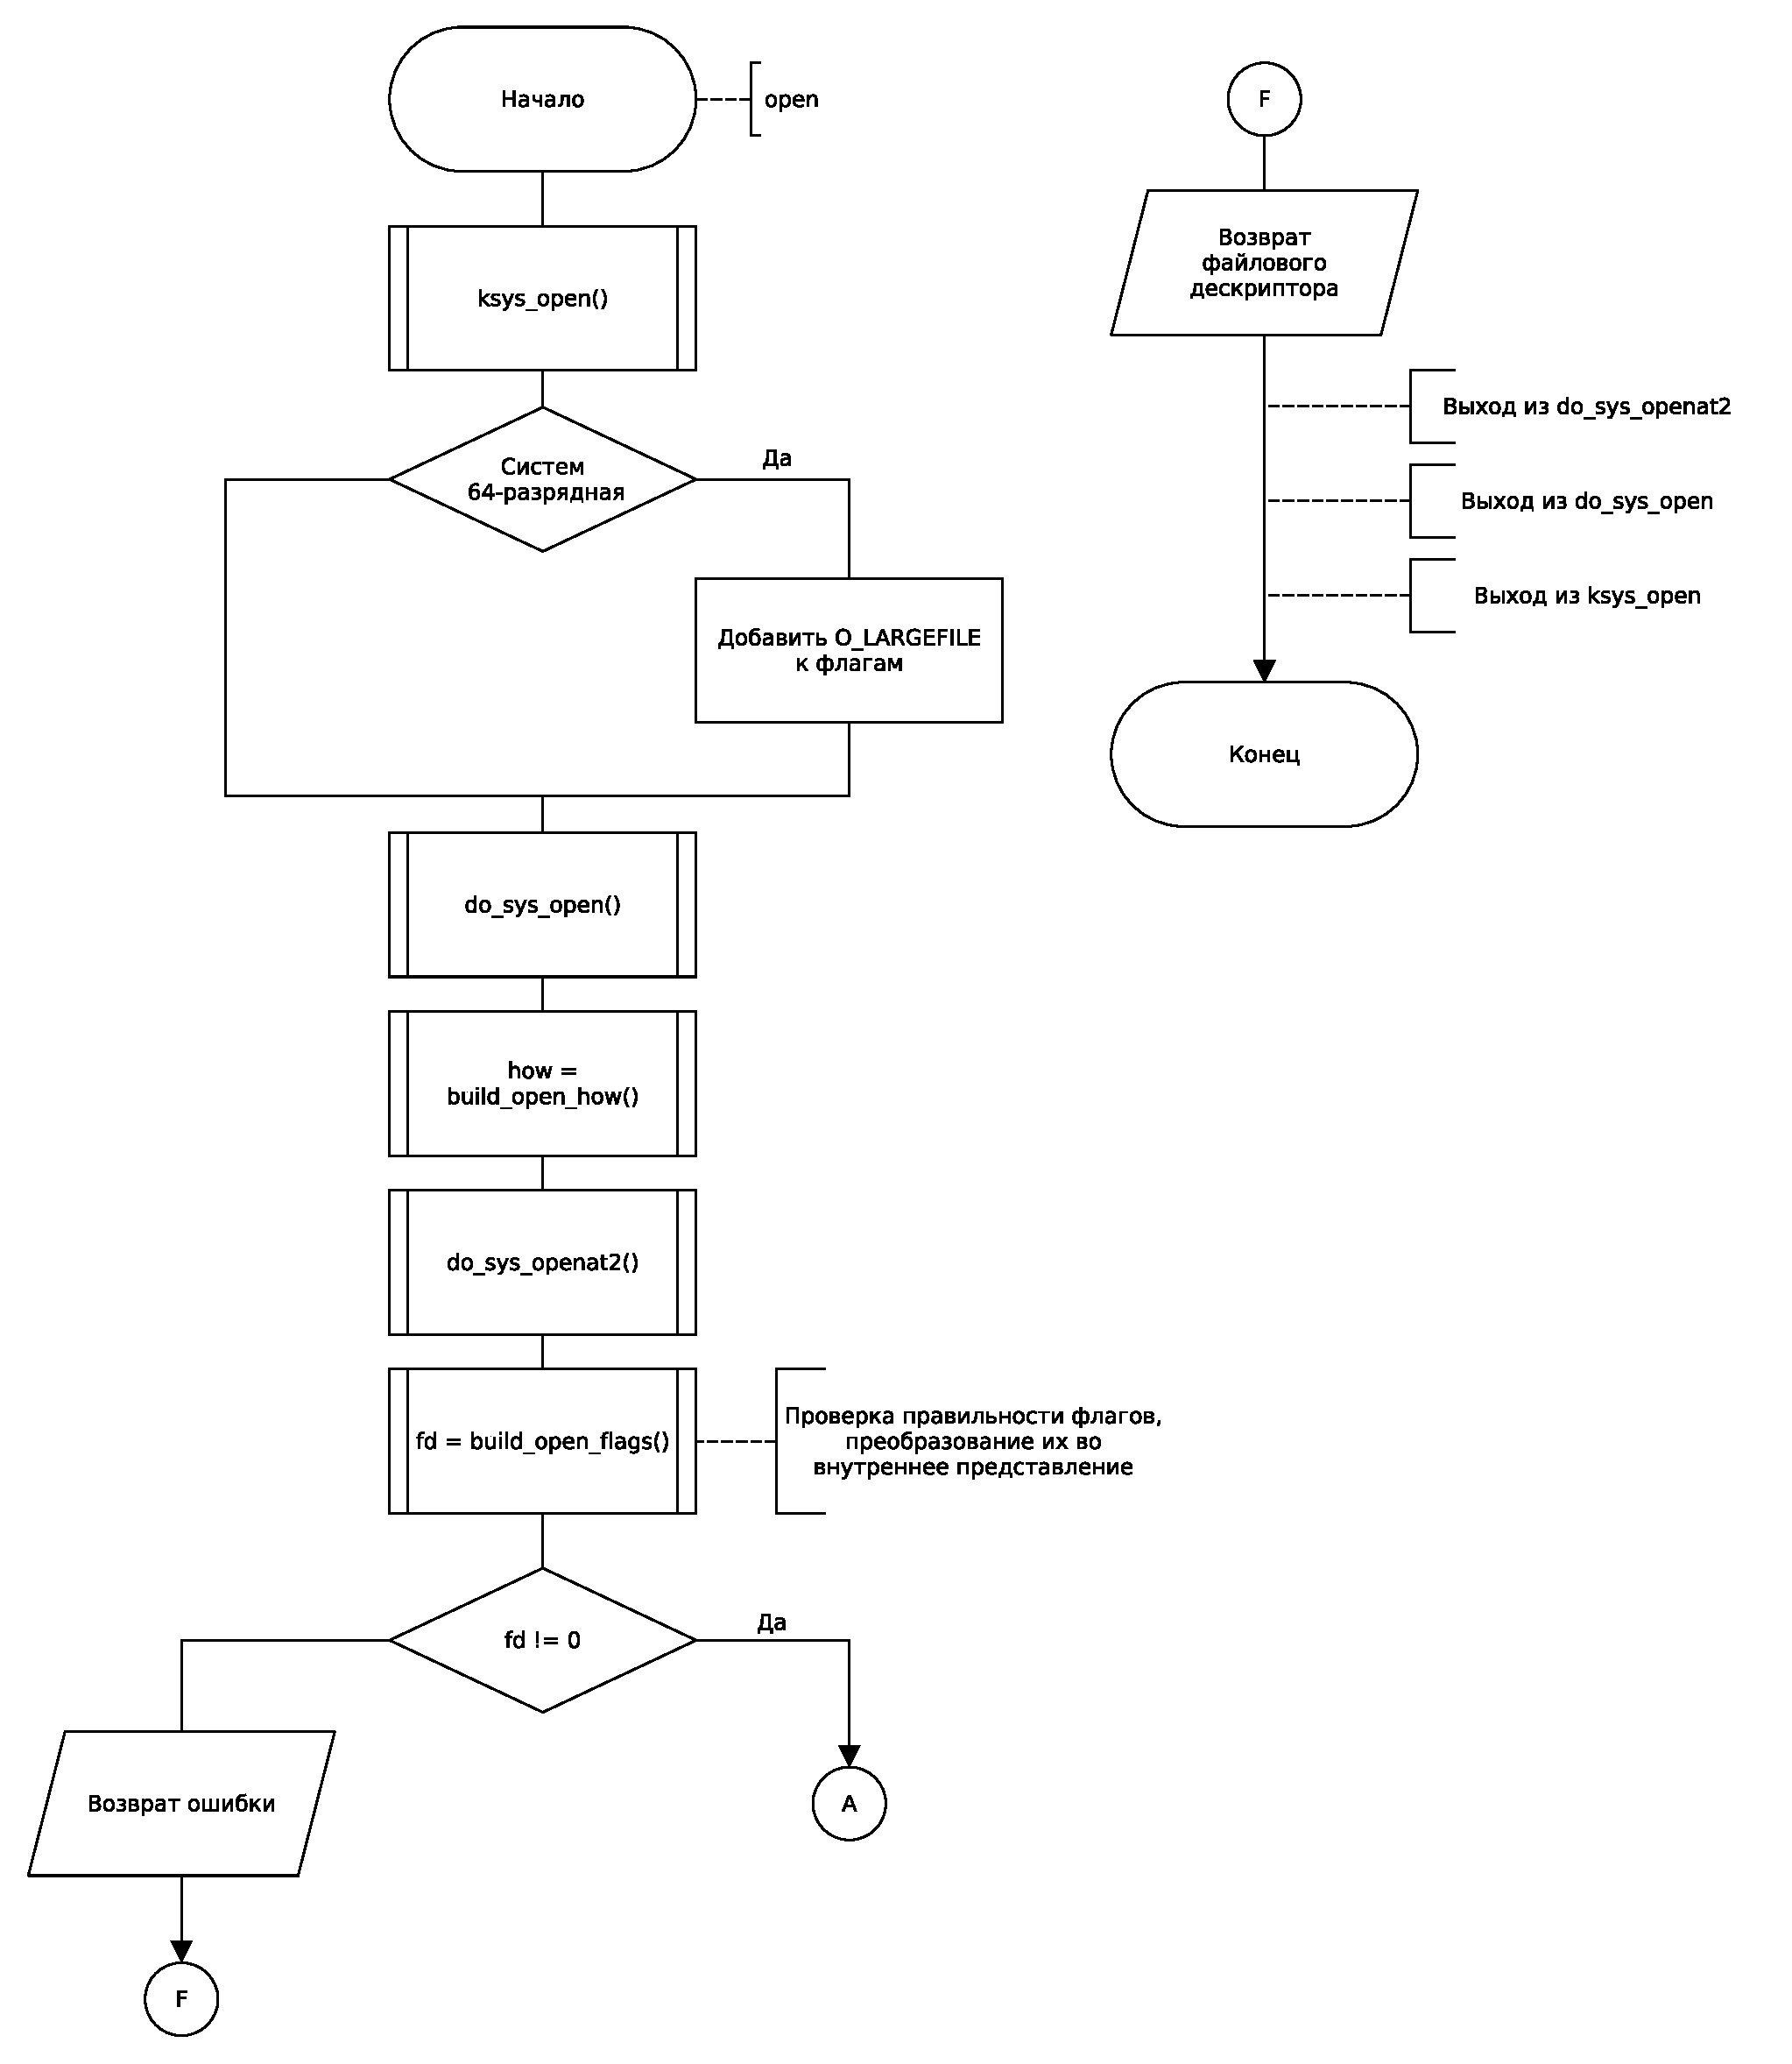
\includegraphics[scale=0.5]{pdf/flowchart01.pdf}
\end{figure}
\begin{figure}[H]
    \centering
    \caption{}
    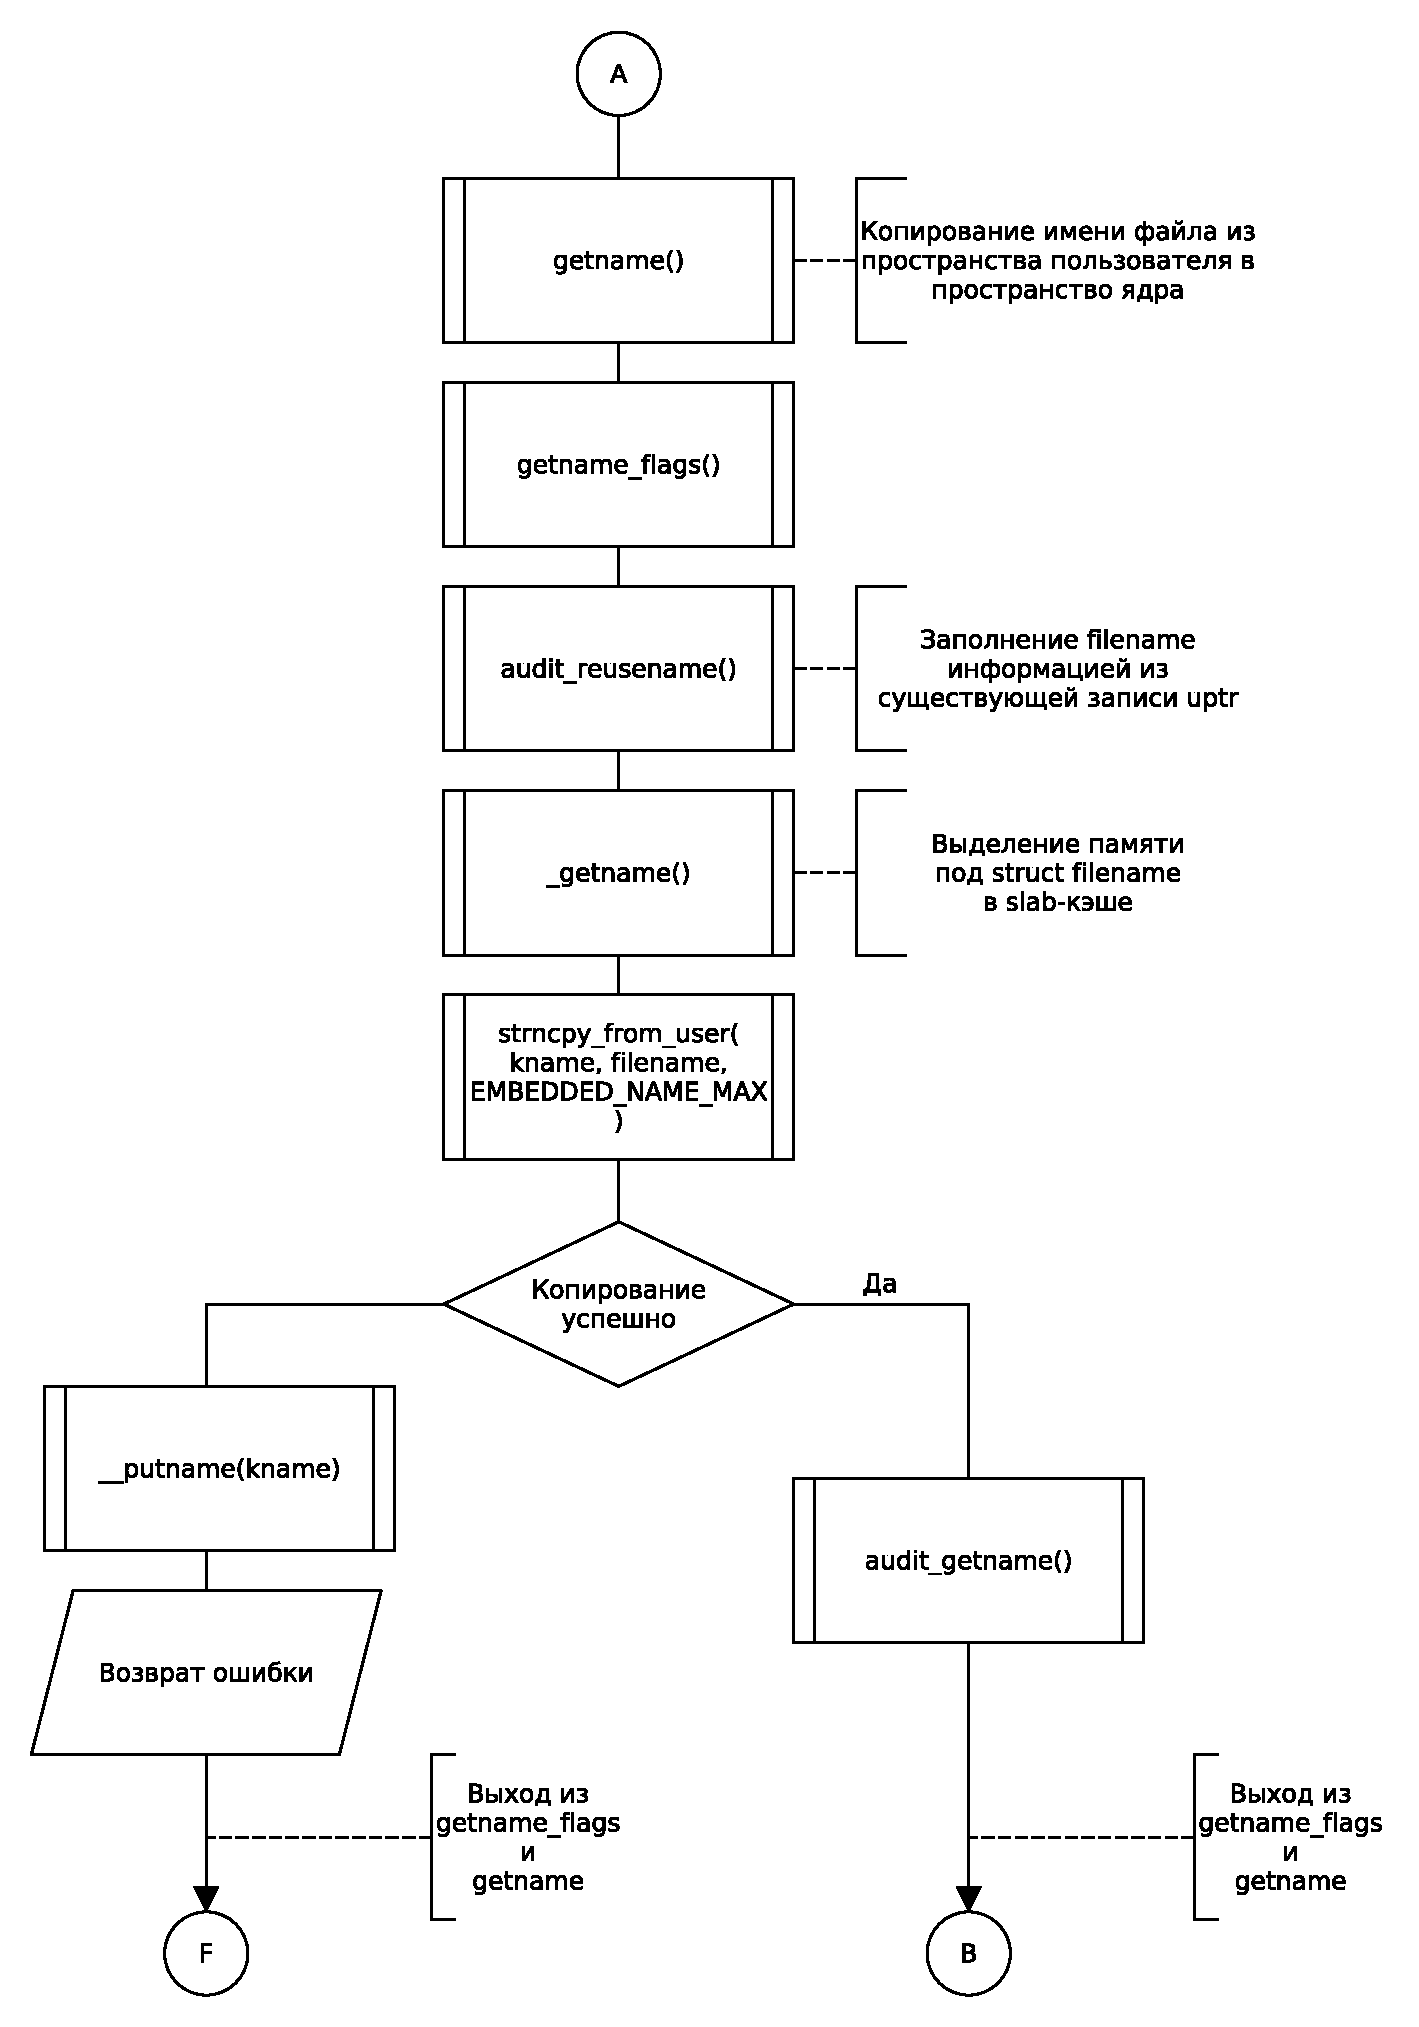
\includegraphics[scale=0.5]{pdf/flowchart02.pdf}
\end{figure}
\begin{figure}[H]
    \centering
    \caption{}
    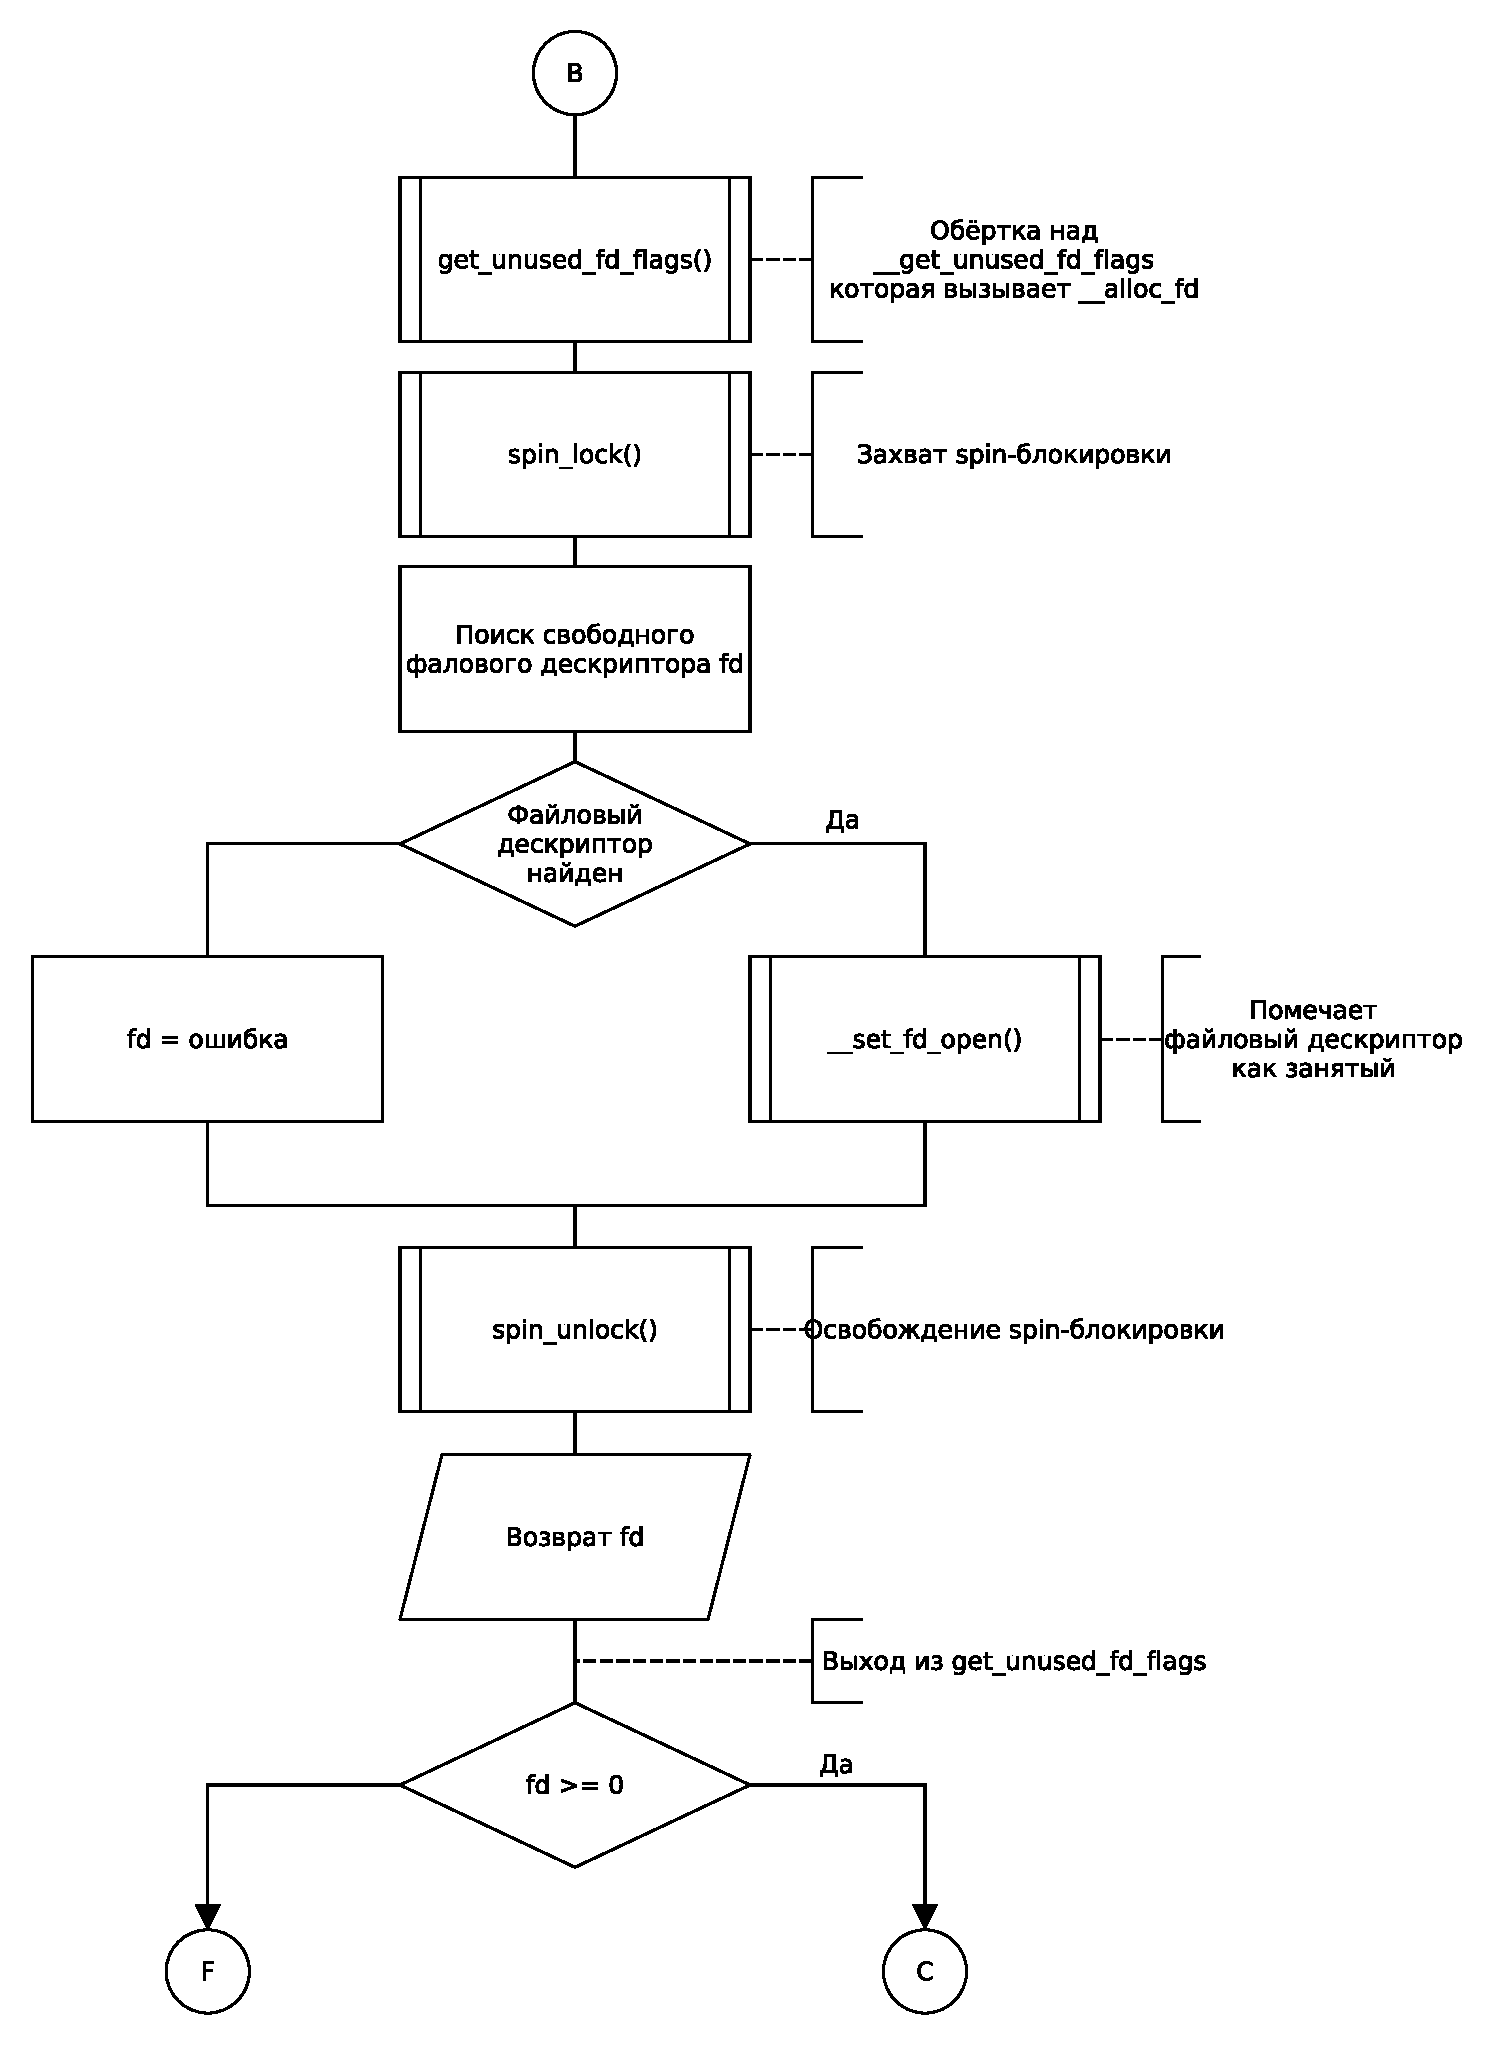
\includegraphics[scale=0.5]{pdf/flowchart03.pdf}
\end{figure}
\begin{figure}[H]
    \centering
    \caption{}
    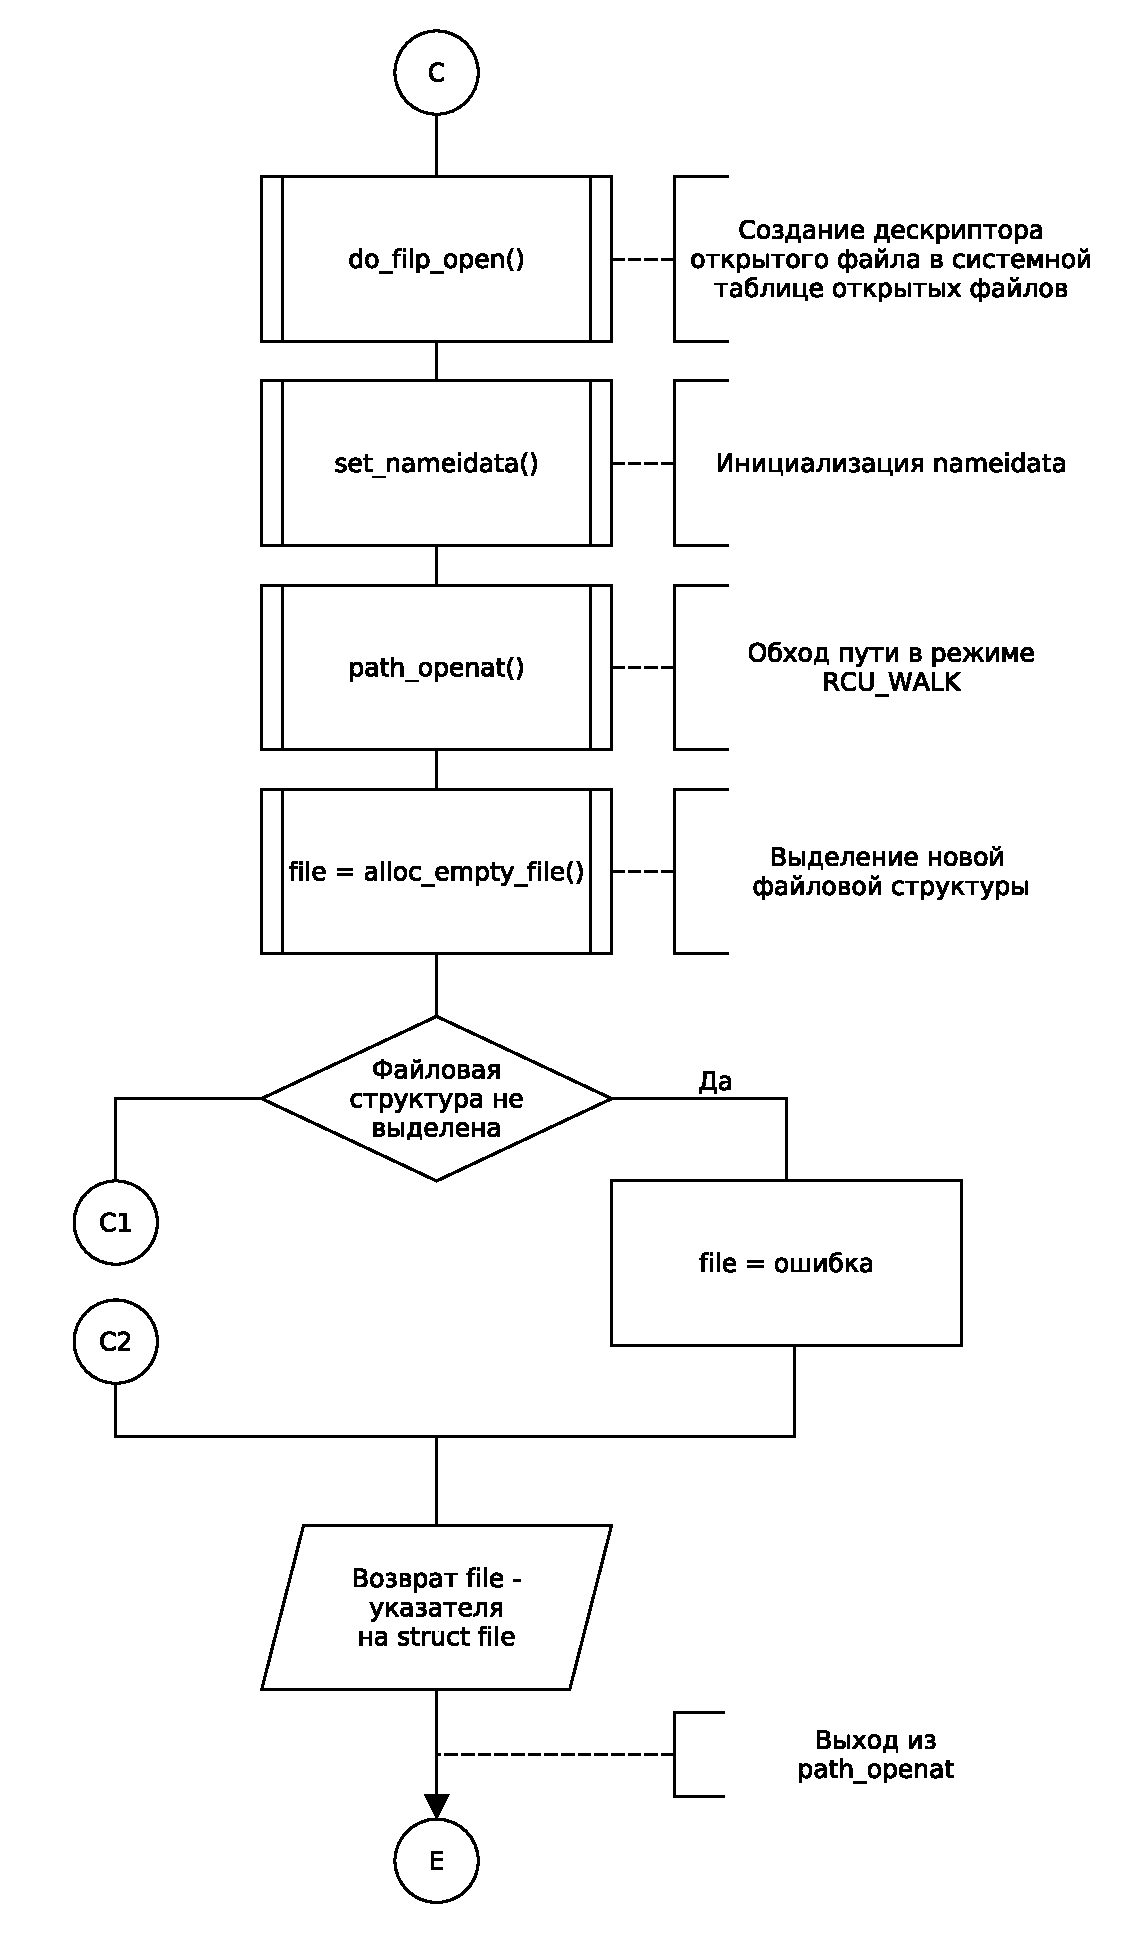
\includegraphics[scale=0.5]{pdf/flowchart04.pdf}
\end{figure}
\begin{figure}[H]
    \centering
    \caption{}
    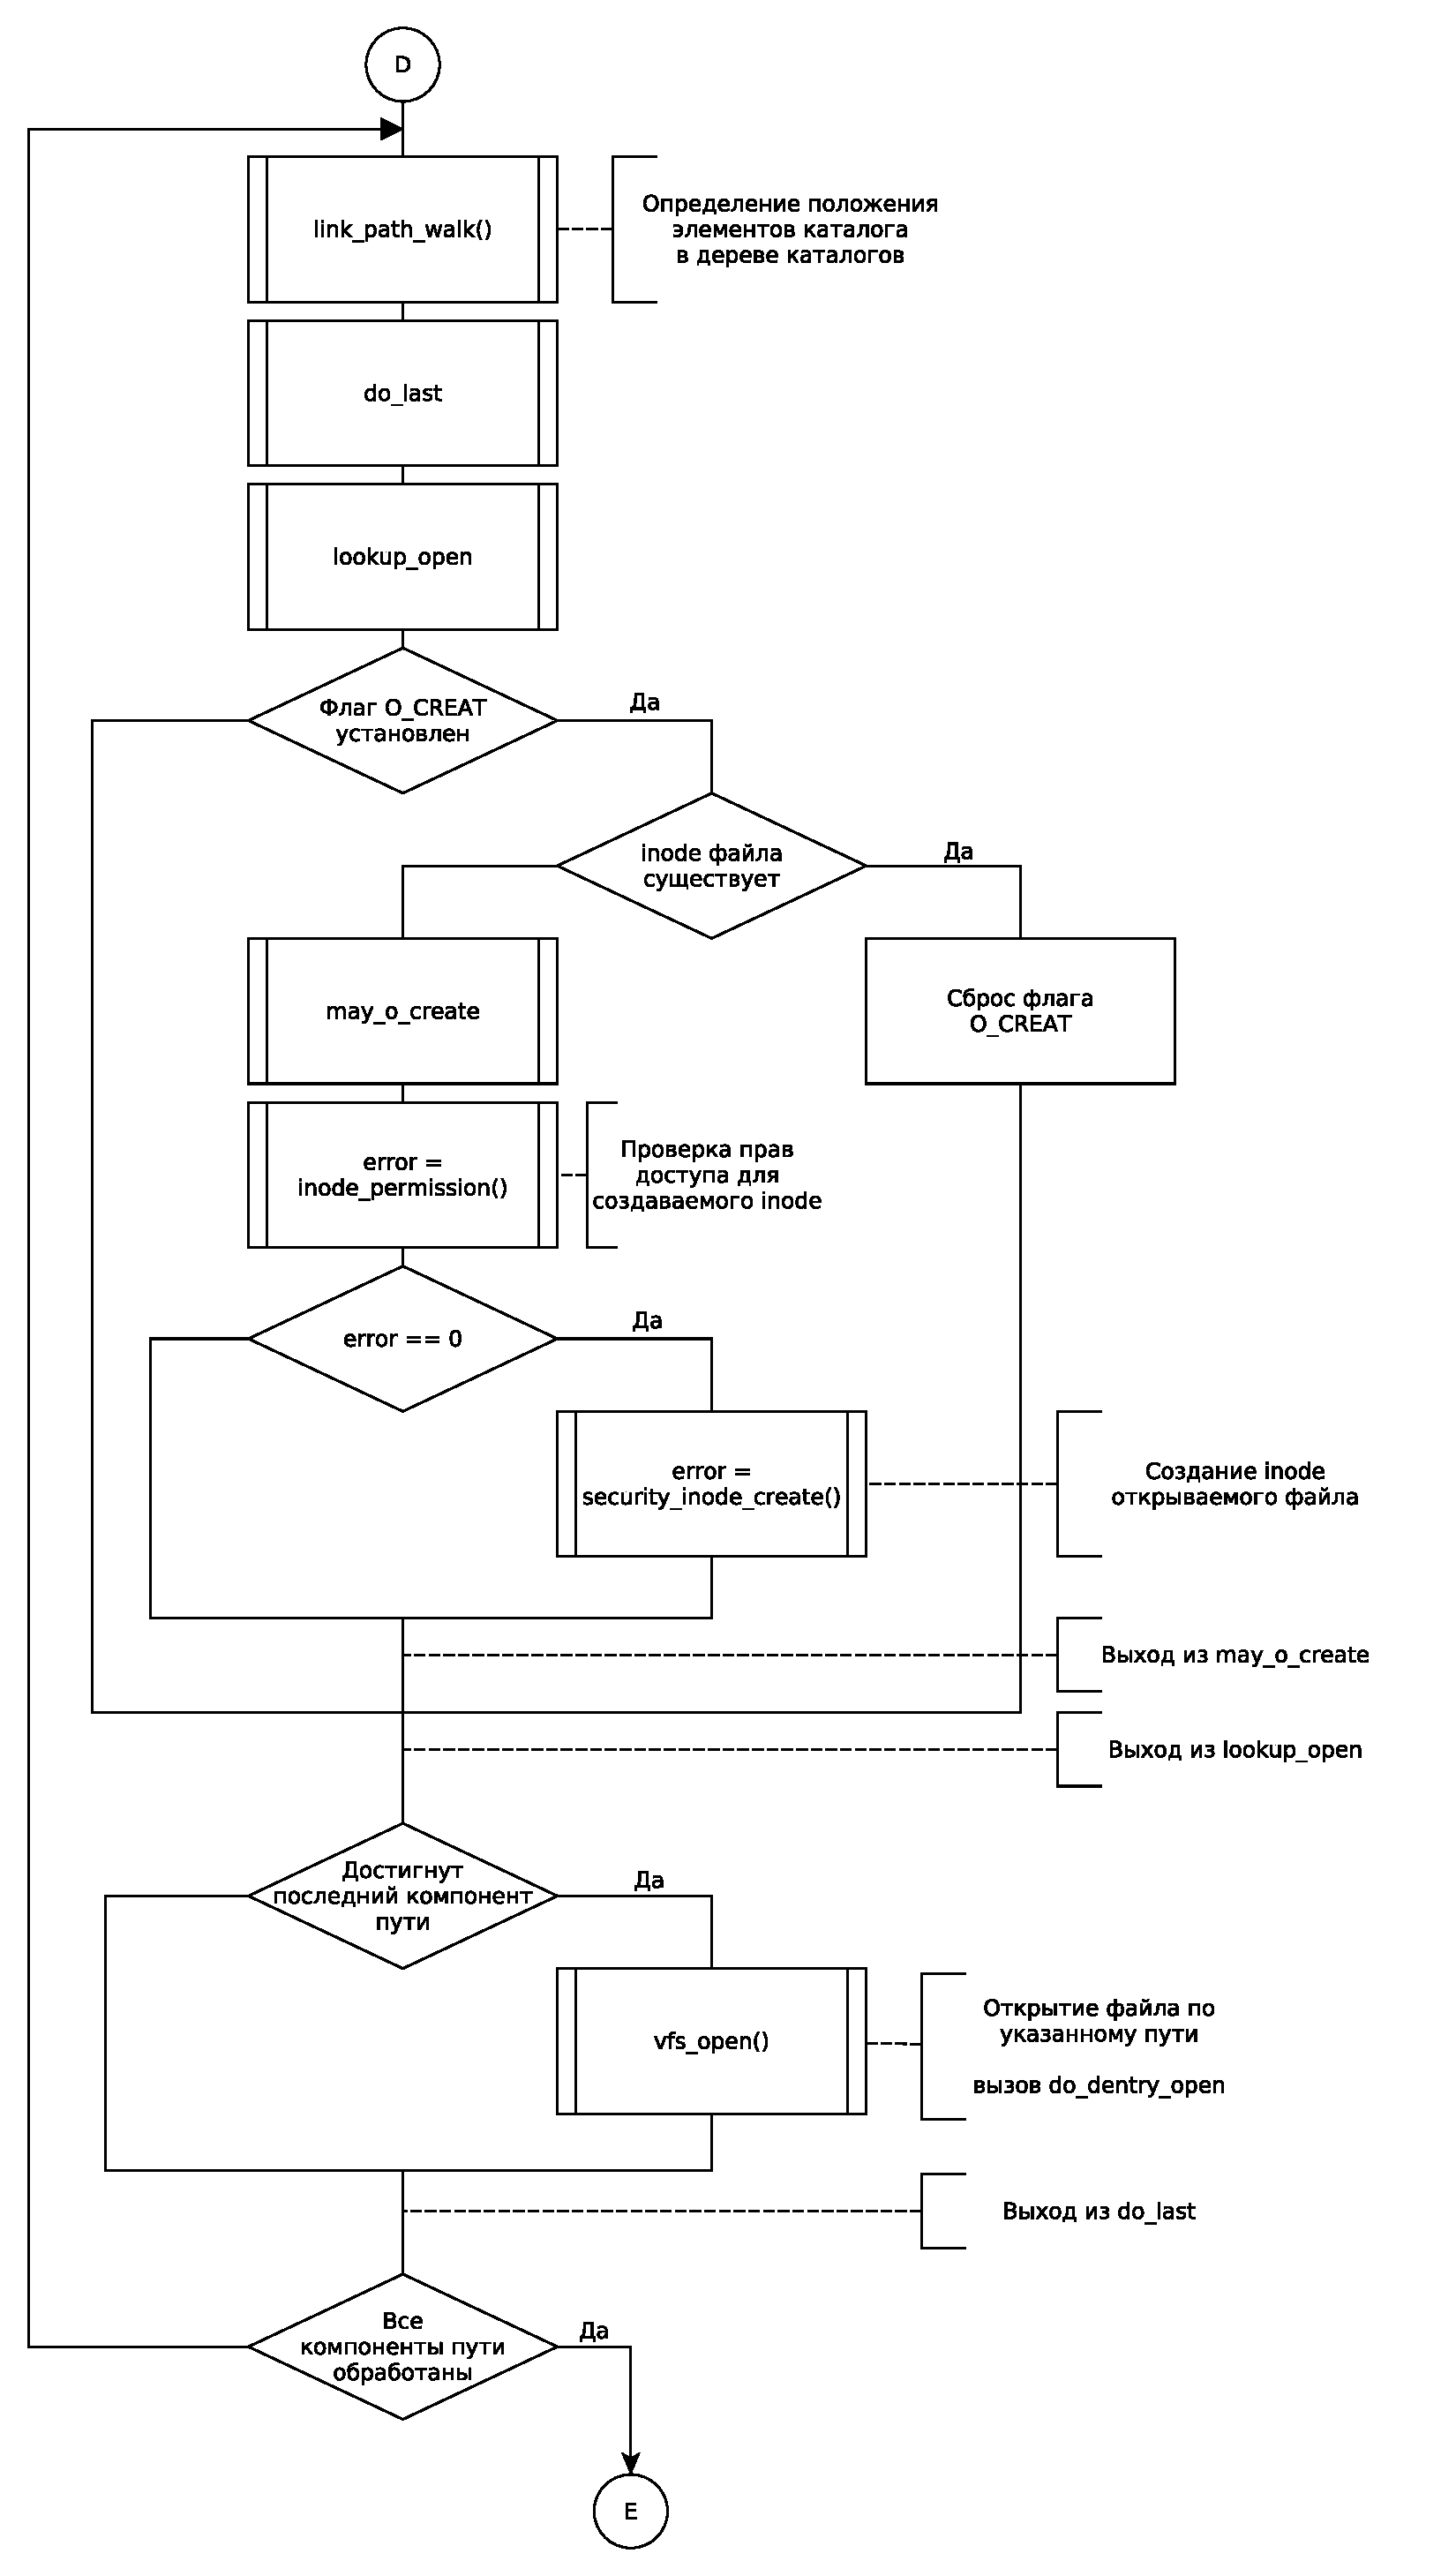
\includegraphics[scale=0.5]{pdf/flowchart05.pdf}
\end{figure}
\begin{figure}[H]
    \centering
    \caption{}
    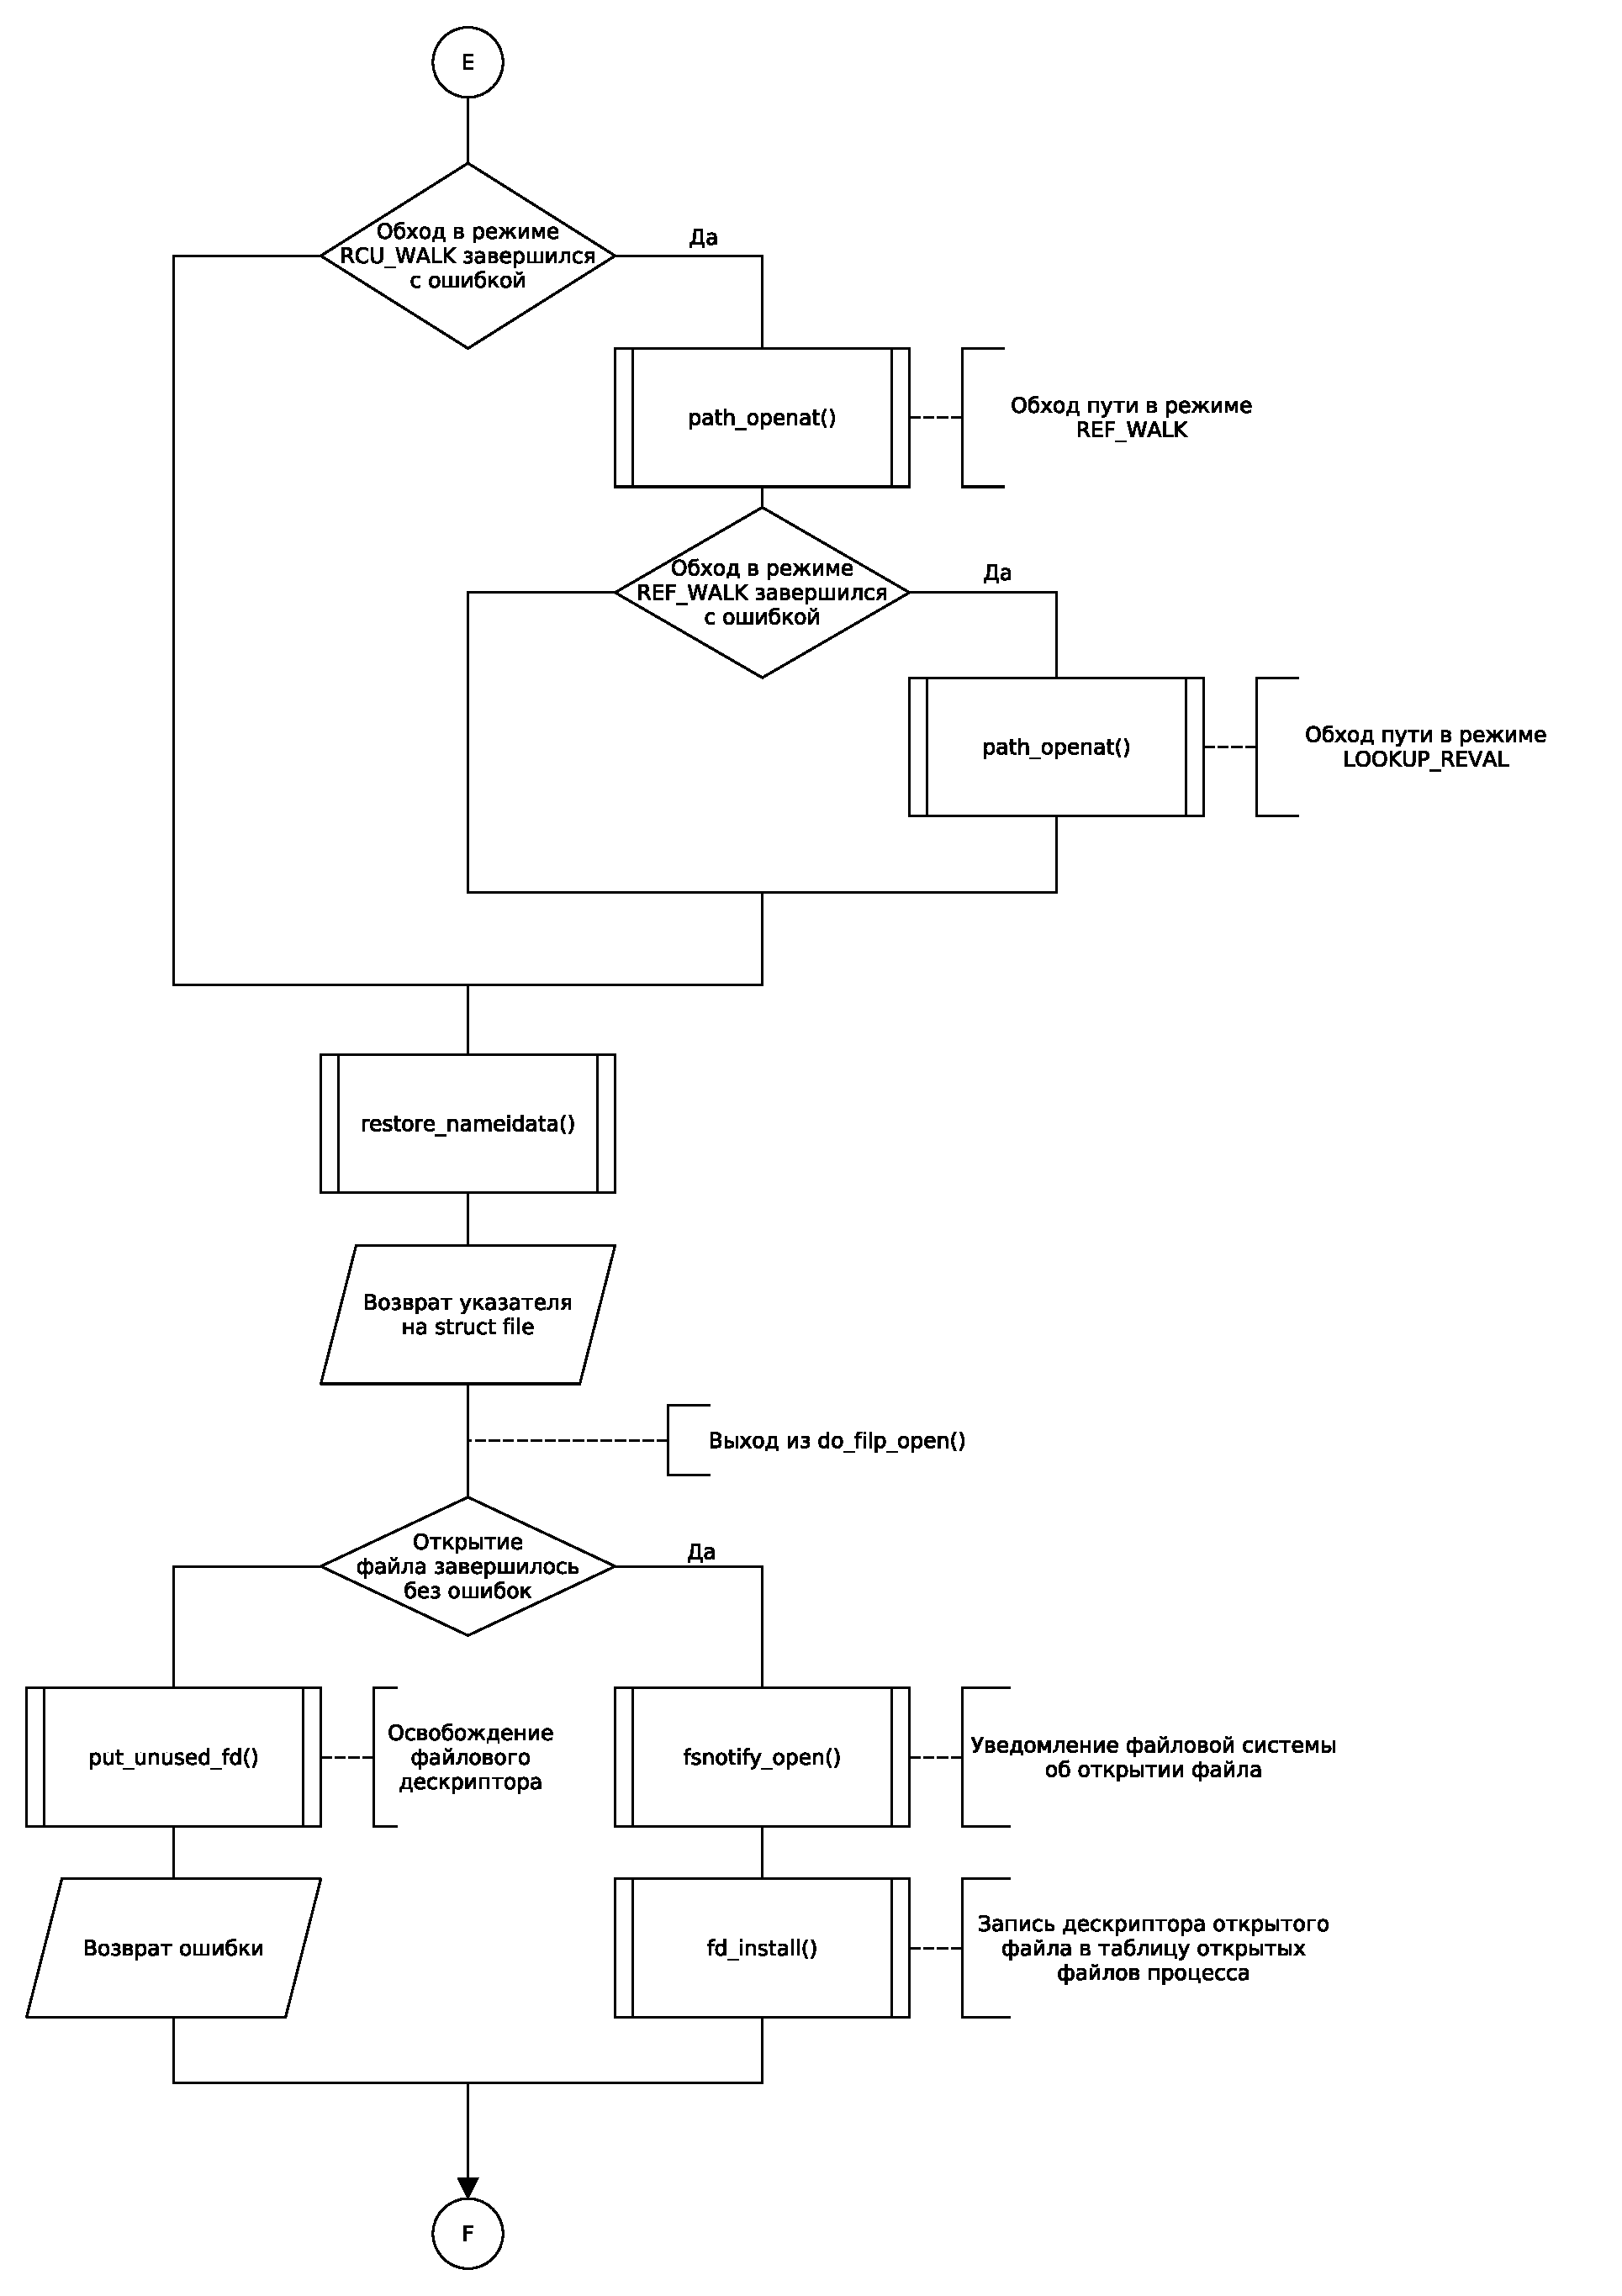
\includegraphics[scale=0.5]{pdf/flowchart06.pdf}
\end{figure}

